\setcounter{page}{2}

\chapter*{Введение}
\addcontentsline{toc}{chapter}{Введение}

Практикум посвящен освоению принципов работы вычислительного комплекса 
Тераграф и получению практических навыков решения задач обработки 
множеств на основе гетерогенной вычислительной структуры. В ходе 
практикума необходимо ознакомиться с типовой структурой двух 
взаимодействующих программ: хост-подсистемы и программного ядра 
sw\_kernel. Участникам предоставляется доступ к удаленному серверу с 
ускорительной картой и настроенными средствами сборки проектов, 
конфигурационный файл для двухъядерной версии микропроцессора Леонард 
Эйлер, а также библиотека leonhard x64 xrt c открытым исходным кодом.

\chapter{Сведения о взаимодействии \\хост-подсистемы и программного ядра sw\_kernel}
Рассмотрим следующие примеры кода подсистемы и программного ядра, которые мы будем использовать в практикуме. Пример выполняет следующие действия:

\begin{enumerate}
	\item Хост-подсистема инициализирует ядра GPC: \\lnh\_inst.load\_sw\_kernel(argv[2], group, core);, после чего становится возможным запуск обработчиков программного ядра sw\_kernel. В практикуме используется версия микропроцессора Леонард Эйлер с одной группой и двумя ядрами GPC, при этом в файле gpc\_defs.h разрешено использование только ядра \#0 группы \#0 (настройка может быть изменена пользователем).
	\item Хост-подсистема выделяет память под буферы \\gpc2host\_buffer и host2gpc\_buffer
	\item В буфере host2gpc\_buffer инициализируется массив ключей и значений для записи в GPC.
	\item Запускается обработчик insert\_burst и запускается механизм прямого доступа к памяти для записи host2gpc\_buffer в глобальную память группы \#0. Последовательность указанных действий может быть обратной: сначала может быть запущен механизм DMA, после чего запускается обработчик.
	\item Хост-подсистема ожидает завершения копирования памяти \\(buf\_write\_join) для синхронизации процессов.
	\item Хост-подсистема передает сообщение с количеством ключей и значений (m\_send(…)).
	\item Программное ядро в обработчике insert\_burst получает сообщение и выделяет буфер (buffer) для хранения данных в RAM CPE.
	\item Программное ядро копирует данные в буфер и последовательно вызывает команду INS микропроцессора lnh64: \\lnh\_ins\_sync(TEST\_STRUCTURE,buffer[2*i],buffer[2*i+1]).
	\item Последовательность действий для реализации пакетной обработки Последовательность действий для реализации пакетной обработки
	\item Далее происходит запуск обработчика для последовательного обхода множества ключей и выдачи их обратно в хост-подсистему.
	\item Программное ядро в обработчике search\_burst получает количество ключей в структуре \\(unsigned int count = lnh\_get\_num(TEST\_STRUCTURE))
	\item Обход структуры начинается с выборки минимального ключа \\(lnh\_get\_first(TEST\_STRUCTURE))
	\item Далее осуществляется запись ключа и значения в буфер для обратной передачи в хост-подсистему.
	\item Используя итерационный цикл, или же проверяя результат выполнения функции lnh\_next(TEST\_STRUCTURE,lnh\_core.result.key) цикл повторяется до обхода всей структуры TEST\_STRUCTURE.
	\item Альтернативно может быть использован следующий код для последовательного обхода структуры.
\captionsetup{singlelinecheck = false, justification=raggedright}
\begin{lstlisting}[label=code, caption=Код последовательного обхода структуры]
	 lnh_get_first(TEST_STRUCTURE);
	 do {
		//lnh_core.result.key   - found key
		//lnh_core.result.value - found value
		...
	 } while (lnh_next(TEST_STRUCTURE,lnh_core.result.key));
\end{lstlisting}
\captionsetup{singlelinecheck = false, justification=centering}

	\item По завершению обхода программное ядро посылает сообщение с количеством переданных ключей и значений.
	\item Хост-подсистема ожидает получения сообщения, после чего последовательно проверяет, что ключ в буфере совпадает с ожидаемым.
	\item В итоге выдается сообщение о результате тестирования.
\end{enumerate}

\chapter{Выполнение практикума}

Вариант 6

\section{Индивидуальное задание}

Разработать программу для хост-подсистемы и обработчики программного ядра, выполняющие следующие действия.
\\
Сформировать в хост-подсистеме и передать в SPE 256 записей с ключами x и значениями $f(x)=x^2$ в диапазоне значений x от 0 до 1048576. Передать в sw\_kernel числа $x1$ и $x2$ $(x2>x1)$. В хост-подсистему вернуть сумму значений $f(x)$ на диапазоне $(x1,x2)$. Сравнить результат с ожидаемым.

\section{Выполнение индивидуального задания}

Для выполнения индивидуального задания были написаны программы для хост-подсистемы и программного ядра sw\_kernel.

В листингах 2.1 -- 2.2 показан код двух программ -- для хост подсистемы и программного ядра sw\_kernel.

\newpage

\captionsetup{singlelinecheck = false, justification=raggedright}
\begin{lstlisting}[label=code, caption=Код программы host\_main.cpp]
#include <iostream>
#include <stdio.h>
#include <stdexcept>
#include <iomanip>
#ifdef _WINDOWS
#include <io.h>
#else
#include <unistd.h>
#endif


#include "experimental/xrt_device.h"
#include "experimental/xrt_kernel.h"
#include "experimental/xrt_bo.h"
#include "experimental/xrt_ini.h"

#include "gpc_defs.h"
#include "leonhardx64_xrt.h"
#include "gpc_handlers.h"

#define BURST 256

union uint64 {
    uint64_t 	u64;
    uint32_t 	u32[2];
    uint16_t 	u16[4];   
    uint8_t 	u8[8];   
};

uint64_t rand64() {
    uint64 tmp;
    tmp.u32[0] =  rand();
    tmp.u32[1] =  rand();
    return tmp.u64;
}

static void usage()
{
	std::cout << "usage: <xclbin> <sw_kernel>\n\n";
}

const uint64_t start_ip = 1;

int main(int argc, char** argv)
{
	unsigned int cores_count = 0;
	float LNH_CLOCKS_PER_SEC;


	//Assign xclbin
	if (argc < 3) {
		usage();
		throw std::runtime_error("FAILED_TEST\nNo xclbin specified");
	}

	//Open device #0
	leonhardx64 lnh_inst = leonhardx64(0,argv[1]);
	lnh_inst.load_sw_kernel(argv[2], 0, 0);


	//Выделение памяти под буферы gpc2host и host2gpc для каждого ядра и группы
	uint64_t *host2gpc_buffer = (uint64_t*) malloc(2*BURST*sizeof(uint64_t));
	uint64_t *gpc2host_buffer = (uint64_t*) malloc(2*BURST*sizeof(uint64_t));
	
	uint64_t x1, x2;
	std::cout << "Input x1, x2 (256 >= x2 > x1 >= 0):" << std::endl;
	std::cin >> x1 >> x2;

	if (!(x1 >= 0 && x1 < x2 && x2 < 256)) 
	{
		std::cout << "Error: incorrect x1, x2" << std::endl;
		return 1;
	}

	//Создание массива ключей и значений для записи в lnh64
	for (int i = 0; i < BURST ; i++) 
	{
		host2gpc_buffer[2*i] = i;
		//Второй uint64_t - value
		host2gpc_buffer[2*i+1] =  i * i;
		// std::cout << host2gpc_buffer[2*i] << " " << host2gpc_buffer[2*i+1] << std::endl; 
	}

	//Запуск обработчика insert_burst
	lnh_inst.gpc[0][0]->start_async(__event__(insert_burst));

	//DMA запись массива host2gpc_buffer в глобальную память
	lnh_inst.gpc[0][0]->buf_write(BURST*2*sizeof(uint64_t),(char*)host2gpc_buffer);

	//Ожидание завершения DMA
	lnh_inst.gpc[0][0]->buf_write_join();

	//Передать количество key-value и наш ключ
	lnh_inst.gpc[0][0]->mq_send(BURST);
	lnh_inst.gpc[0][0]->mq_send(x1);
	lnh_inst.gpc[0][0]->mq_send(x2);

	//Запуск обработчика для последовательного обхода множества ключей
	lnh_inst.gpc[0][0]->start_async(__event__(search_burst));

	//Получить количество ключей и значение по переданному ключу
	unsigned int count;
	uint64_t result;

	count = lnh_inst.gpc[0][0]->mq_receive();
	result = lnh_inst.gpc[0][0]->mq_receive();

	//Прочитать количество ключей
	lnh_inst.gpc[0][0]->buf_read(count * 2 * sizeof(uint64_t), (char*)gpc2host_buffer);

	//Ожидание завершения DMA
	lnh_inst.gpc[0][0]->buf_read_join();

	//Чтение значения, полученного по ключу и проверка целостности данных
	x2--;
	uint64_t answer = x2 * (x2 + 1) * (2 * x2 + 1) / 6 - x1 * (x1 + 1) * (2 * x1 + 1) / 6;
	std::cout << "Your integral: " << result << std::endl << "Expected: " << answer << std::endl; 

	if (result == answer) 
		std::cout << "(CORRECT)" << std::endl;
	else
		std::cout << "(INCORRECT)" << std::endl;

	free(host2gpc_buffer);
	free(gpc2host_buffer);
	return 0;
}
\end{lstlisting}
\captionsetup{singlelinecheck = false, justification=centering}


\newpage

\captionsetup{singlelinecheck = false, justification=raggedright}
\begin{lstlisting}[label=code, caption=Код программы sw\_kernel\_main.c]
/*
 * gpc_test.c
 *
 * sw_kernel library
 *
 *  Created on: April 23, 2021
 *      Author: A.Popov
 */

#include <stdlib.h>
#include <unistd.h>
#include "lnh64.h"
#include "gpc_io_swk.h"
#include "gpc_handlers.h"

#define SW_KERNEL_VERSION 26
#define DEFINE_LNH_DRIVER
#define DEFINE_MQ_R2L
#define DEFINE_MQ_L2R
#define __fast_recall__

#define TEST_STRUCTURE 1

extern lnh lnh_core;
extern global_memory_io gmio;
volatile unsigned int event_source;

int main(void) {
    /////////////////////////////////////////////////////////
    //                  Main Event Loop
    /////////////////////////////////////////////////////////
    //Leonhard driver structure should be initialised
    lnh_init();
    //Initialise host2gpc and gpc2host queues
    gmio_init(lnh_core.partition.data_partition);
    for (;;) {
        //Wait for event
        while (!gpc_start());
        //Enable RW operations
        set_gpc_state(BUSY);
        //Wait for event
        event_source = gpc_config();
        switch(event_source) {
            /////////////////////////////////////////////
            //  Measure GPN operation frequency
            /////////////////////////////////////////////
            case __event__(insert_burst) : insert_burst(); break;
            case __event__(search_burst) : search_burst(); break;
        }
        //Disable RW operations
        set_gpc_state(IDLE);
        while (gpc_start());

    }
}

//-------------------------------------------------------------
//      Получить пакет из глобальной памяти и аписат в lnh64
//-------------------------------------------------------------
 
void insert_burst() {

    //Удаление данных из структур
    lnh_del_str_sync(TEST_STRUCTURE);
    //Объявление переменных
    unsigned int count = mq_receive();
    unsigned int size_in_bytes = 2*count*sizeof(uint64_t);
    //Создание буфера для приема пакета
    uint64_t *buffer = (uint64_t*)malloc(size_in_bytes);
    //Чтение пакета в RAM
    buf_read(size_in_bytes, (char*)buffer);
    //Обработка пакета - запись 
    for (int i=0; i<count; i++) {
        lnh_ins_sync(TEST_STRUCTURE,buffer[2*i],buffer[2*i+1]);
    }
    lnh_sync();
    free(buffer);
}


void search_burst() {
    //Ожидание завершения предыдущих команд
    lnh_sync(); 
    //Объявление переменных
    unsigned int count = lnh_get_num(TEST_STRUCTURE);
    //Передать количество key-value
    mq_send(count);
    //Получить ключ
    auto x1 = mq_receive();
    auto x2 = mq_receive();
    //Поиск по ключу
    
    lnh_grls_sync(x1, x2, 1, 2);
    uint64_t n = lnh_get_num(2);
    lnh_get_first(2);
    uint64_t sum = lnh_core.result.value;
    for (int i = 0; i < n - 1; i++)
	{
        lnh_next(2, lnh_core.result.key);
        sum += lnh_core.result.value;
    }
    //Отправка ответа
	mq_send(sum);
    // mq_send(buffer[2*1+1]);
}
\end{lstlisting}
\captionsetup{singlelinecheck = false, justification=centering}

\newpage
В результате запуска данных программ выводится сумма квадратов между введёнными числами.

\begin{figure}[h!]
	\begin{center}
		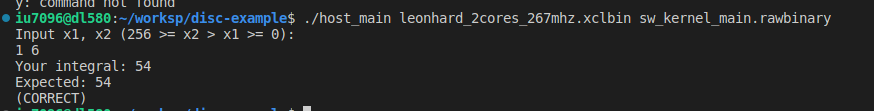
\includegraphics[scale=0.54]{res}
	\end{center}
	\caption{Результат работы программ}
\end{figure}

\chapter*{Заключение}
\addcontentsline{toc}{chapter}{Заключение}

В данном практикуме были освоены принципы работы вычислительного комплекса 
Тераграф и получены практические навыки решения задач обработки 
множеств на основе гетерогенной вычислительной структуры. 

В ходе практикума была изучена структура двух 
взаимодействующих программ: хост-подсистемы и программного ядра 
sw\_kernel. 

Работа проводилась на удаленном сервере с ускорительной 
картой, микропроцессором Леонард Эйлер, а также библиотекой 
leonhard x64 xrt c открытым исходным кодом.

Было выполнено задание согласно индивидуальному варианту.
